\begin{figure}[H]
\centering
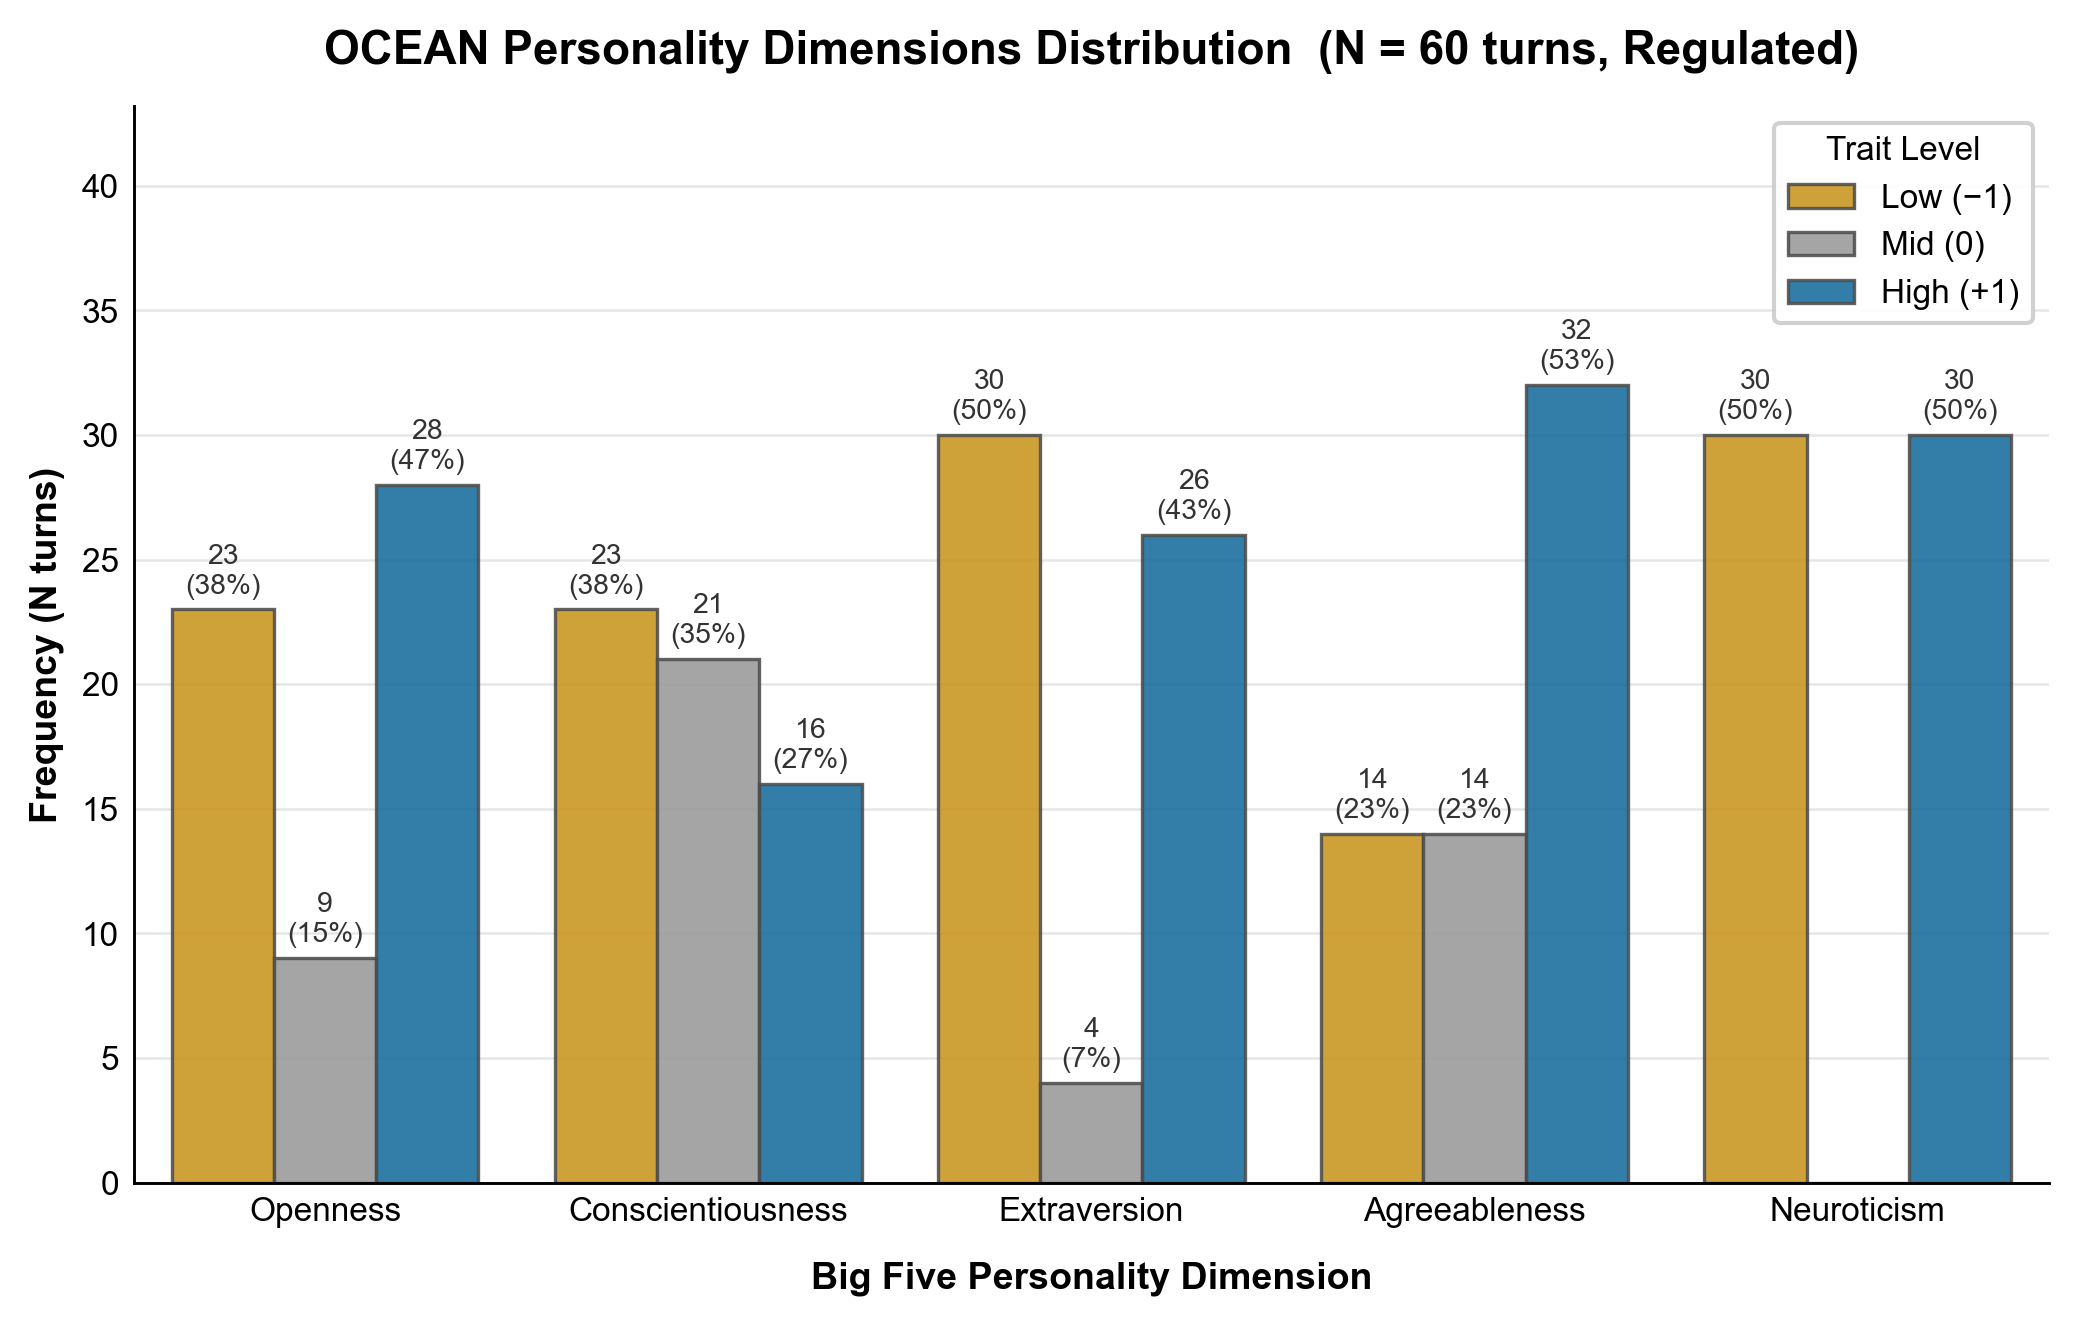
\includegraphics{figures/06_personality_dimensions.png}
\caption{Distribution of detected OCEAN personality dimensions across all conversation turns (Regulated condition, $N = 60$ turns). Grouped bars show frequency of Low ($-1$), Mid ($0$), and High ($+1$) trait levels for each Big Five dimension; values above bars indicate count and percentage. Detection fidelity is dimension-specific: Extraversion, Agreeableness (Type A turns), and Neuroticism show strong alignment ($\geq$87\% intended polarity), while Conscientiousness and Agreeableness (Type B turns) exhibit higher Mid ($0$) rates, reflecting neutral-state assignments when conversational evidence was insufficient. Overall holistic detection accuracy: 98.3\% (59/60 Yes).}
\label{fig:9}
\end{figure}
